\begin{solution}

\begin{enumerate}
\item {[8 points]} The error is shown in the table below.
\begin{center}
\begin{tabular}{r|r}
\hline
\multicolumn{1}{c|}{$N$} & \multicolumn{1}{c}{error} \\ 
\hline
   2  &  2.2920610 \\
   4  &  1.2480270 \\
   8  &  0.6514086 \\
  16  &  0.3327167 \\
  32  &  0.1681236 \\
  64  &  0.0845039 \\
 128  &  0.0423625 \\
 256  &  0.0212089 \\
 512  &  0.0106114
\end{tabular}\end{center} 

The code that generated the results shown in this part, part~(b) and part~(c) is below.

\lstinputlisting{HW8abc.m}

\item {[8 points]} 
The error for the $O(h^2)$ centered difference approximation is shown in the table below.
\begin{center}
\begin{tabular}{r|r}
\hline
\multicolumn{1}{c|}{$N$} & \multicolumn{1}{c}{error} \\
\hline
   2 &  0.4117528 \\
   4 &  0.1461393 \\
   8 &  0.0448560 \\
  16 &  0.0125498 \\
  32 &  0.0033288 \\
  64 &  0.0008579 \\
 128 &  0.0002178 \\
 256 &  0.0000549 \\
 512 &  0.0000138
\end{tabular}\end{center}

\item {[5 points]} The errors for the approximation in part~(b) decay much more rapidly than the errors for the approximation in part~(a).
This is made clear by the plot below.

\begin{center}
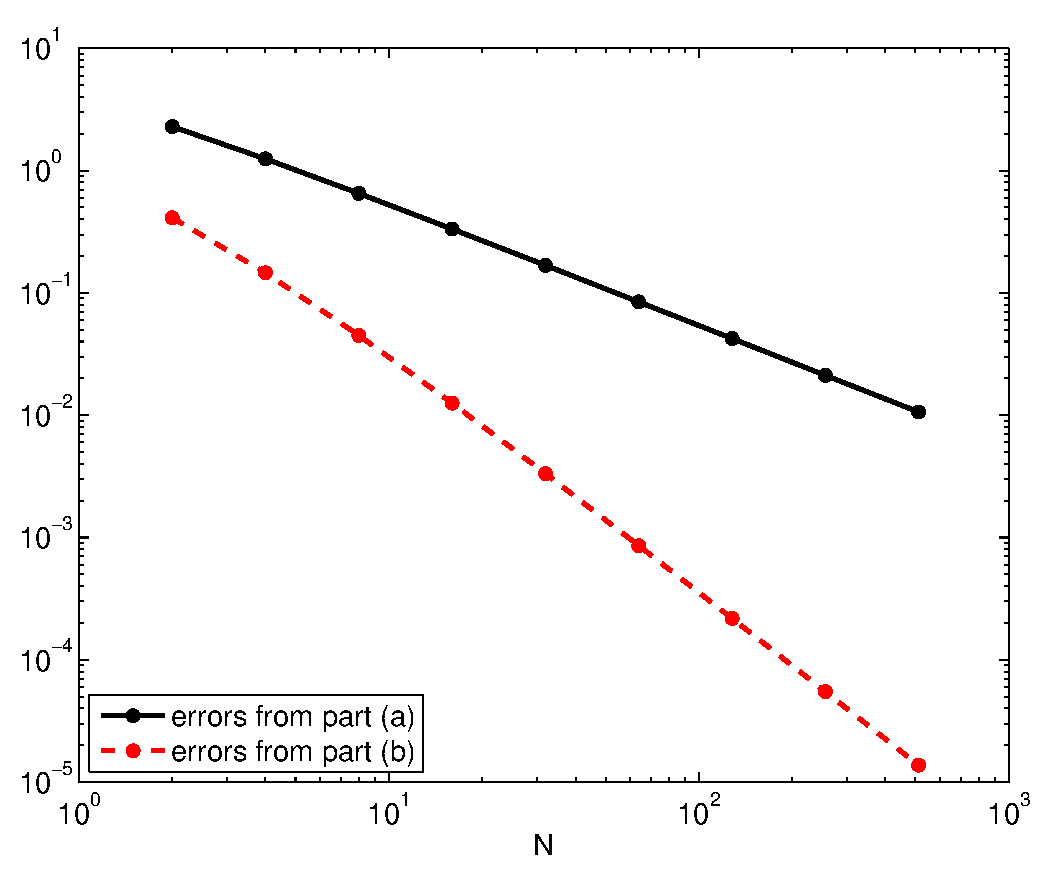
\includegraphics[scale=0.7]{findiff}
\end{center}

\item {[4 points]} Roughly speaking, the forward difference requires $N\approx 512$ 
before it is accurate to two digits, while the centered difference only requires 
$N\approx 16$.   (When used in the context of solving differential equations,
the improved accuracy of the centered difference formula allows one to work
with smaller matrices than required for the forward difference formula,
potentially delivering a great speed-up in run-time.)

\end{enumerate}


\end{solution}
